\documentclass[letterpaper,11pt,landscape]{article}
%\usepackage[margin=0.25in]{geometry}
\documentclass[11pt]{article}
\usepackage[paperheight=6.5in,paperwidth=11.5in,margin=0.25in]{geometry}
\usepackage{xspace}

% Use sans serif font for readability
\usepackage[T1]{fontenc}
\usepackage{lmodern}
\renewcommand{\familydefault}{\sfdefault}
%\usepackage[utf8]{inputenc}

\usepackage{tikz}
\usetikzlibrary{shapes.geometric, arrows}

\tikzstyle{input} = [rectangle, rounded corners, minimum width=3cm, minimum height=1cm,text centered, draw=black, fill=red!30,text width=2.5cm]
\tikzstyle{io} = [trapezium, trapezium left angle=70, trapezium right angle=110, minimum width=3cm, minimum height=1cm, text centered, draw=black, fill=blue!30, text width=2.5cm]
\tikzstyle{catalog} = [rectangle, minimum width=3cm, minimum height=1cm, text centered, draw=black, fill=orange!30]
\tikzstyle{decision} = [diamond, minimum width=3cm, minimum height=1cm, text centered, draw=black, fill=green!30]
\tikzstyle{arrow} = [thick,->,>=stealth]
%\tikzstyle{edge} = [width=1.8pt]
\tikzstyle{textbox} = [rectangle, minimum width=3cm, minimum height=1cm, text centered, draw=white,text width=3cm]	

% Commands
\newcommand{\code}[1]{\texttt{#1}\xspace}
\newcommand{\ngmix}{\code{ngmix}}
\newcommand{\balrog}{\code{Balrog}}
\newcommand{\sompz}{\code{SOMpz}}
\newcommand{\mofsof}{\code{MOF/SOF}}
\newcommand{\dnf}{\code{DNF}}
\newcommand{\bpz}{\code{BPZ}}
\newcommand{\metacal}{\code{metacal}}
\newcommand{\sextractor}{\code{SourceExtractor}}

\begin{document}

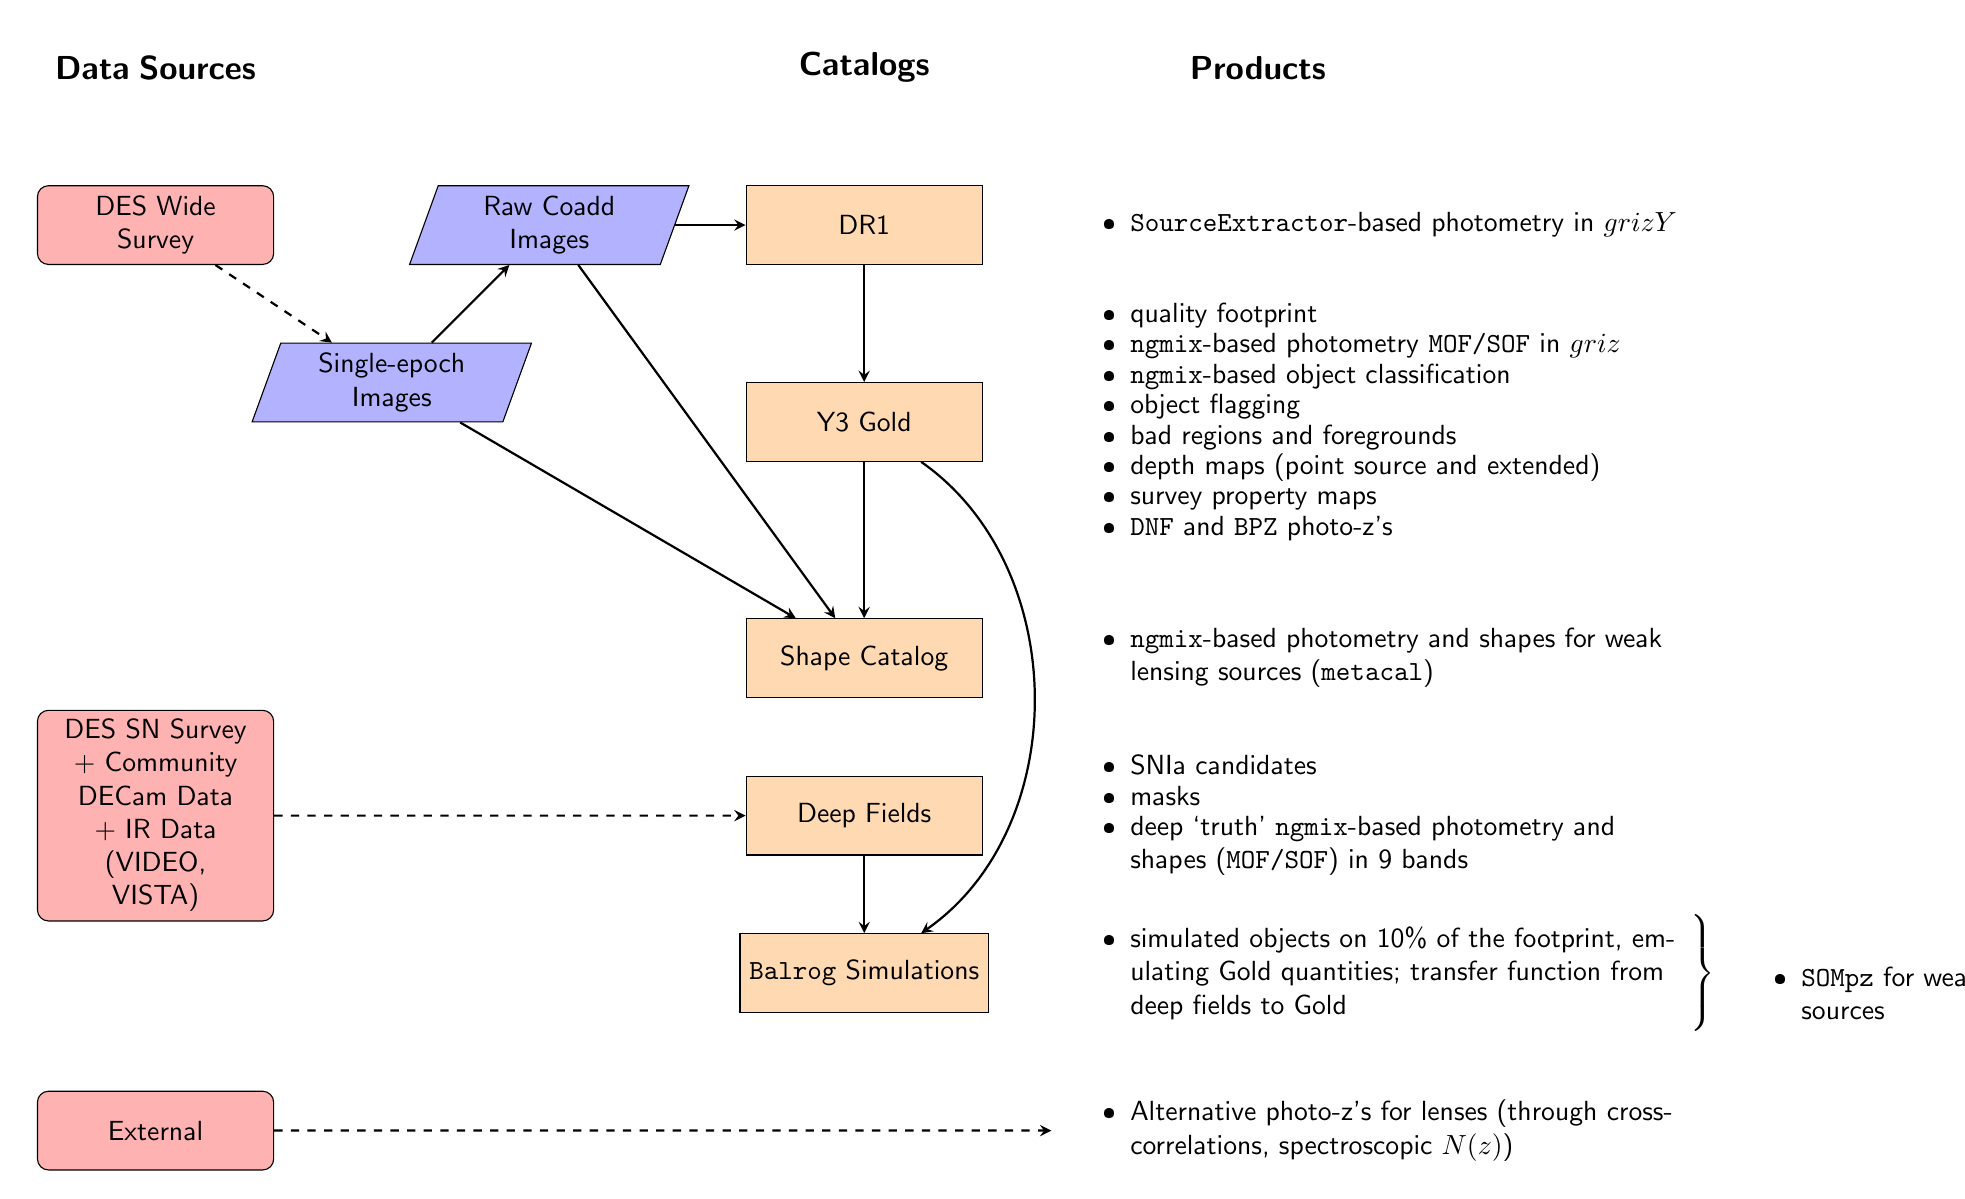
\begin{tikzpicture}[node distance=2cm]

\node (wide) [input]{DES Wide Survey};
\node (sn) [input, below of=wide, yshift=-5.5cm]{DES SN Survey + Community DECam Data + IR Data (VIDEO, VISTA)};
\node (header_survey) [textbox, above of=wide]{\textbf{\large Data Sources}};
\node (se_image) [io, right of=wide, xshift=1cm, yshift=-2cm]{Single-epoch Images};
\node (coadd_image) [io, right of=se_image, xshift=0cm, yshift=2cm]{Raw Coadd Images};
%\node (coadd_image) [io, above of=se_image]{Raw Coadd Images};
\node (dr1) [catalog, right of=coadd_image, xshift=2cm]{DR1};
\node (text_dr1) [textbox, right of=dr1, xshift=2cm]
	{\begin{minipage}{8cm}
	\begin{itemize}\setlength\itemsep{-0.5em}
	 \item \sextractor-based photometry in $grizY$
	 \end{itemize}
	 \end{minipage}};
\node (gold) [catalog, below of=dr1, yshift=-0.5cm]{Y3 Gold};
%\node (text_gold) [textbox, right of=gold, xshift=3cm]{Gold description};
\node (text_gold) [textbox, right of=gold, xshift=2cm]
	{\begin{minipage}{8cm}
	\begin{itemize}\setlength\itemsep{-0.5em}
	 \item quality footprint
	 \item \ngmix-based photometry \mofsof in $griz$
	 \item \ngmix-based object classification
	 \item object flagging
	 \item bad regions and foregrounds 
	 \item depth maps (point source and extended)
	 \item survey property maps  
	 \item \dnf and \bpz photo-z's
	 \end{itemize}
	 \end{minipage}};
\node (header_catalog) [textbox, above of=dr1]{\textbf{\large Catalogs}};
\node (shape) [catalog, below of=gold, yshift=-1cm]{Shape Catalog};
%\node (text_shape) [textbox, right of=shape, xshift=3cm]{Shape description};
\node (text_shape) [textbox, right of=shape, xshift=2cm]
	{\begin{minipage}{8cm}
	\begin{itemize}\setlength\itemsep{-0.5em}
	 \item \ngmix-based photometry and shapes for weak lensing sources (\metacal)
	 \end{itemize}
	 \end{minipage}};
\node (deep) [catalog, below of=shape]{Deep Fields};
%\node (text_deep) [textbox, right of=deep, xshift=3cm]{Deep description};
\node (text_deep) [textbox, right of=deep, xshift=2cm]
	{\begin{minipage}{8cm}
	\begin{itemize}\setlength\itemsep{-0.5em}
	 \item SNIa candidates 
	 \item masks
	 \item deep `truth' \ngmix-based photometry and shapes (\mofsof) in 9 bands
	 \end{itemize}
	 \end{minipage}};
\node (balrog) [catalog, below of=deep]{\balrog Simulations};
%\node (text_balrog) [textbox, right of=balrog, xshift=3cm]{Balrog description};
\node (text_balrog) [textbox, right of=balrog, xshift=2cm]
	{\begin{minipage}{8cm}
	\begin{itemize}\setlength\itemsep{-0.5em}
	 \item simulated objects on 10\% of the footprint, emulating Gold quantities; transfer function from deep fields to Gold
	 \end{itemize}
	 \end{minipage}};
%\node (text_external) [textbox, below of=text_balrog]{External description};
\node (text_external) [textbox, below of=text_balrog]
	{\begin{minipage}{8cm}
	\begin{itemize}\setlength\itemsep{-0.5em}
	 \item Alternative photo-z's for lenses (through cross-correlations, spectroscopic $N(z)$)
	 \end{itemize}
	 \end{minipage}};
\node (header_product) [textbox, right of=header_catalog, xshift=3cm]{\textbf{\large Products}};
\node (external) [input, below of=sn, yshift=-2cm]{External};
%\node (text_photoz) [textbox, right of=text_balrog, xshift=3cm]{Photo-z description};
\node (text_photoz) [textbox, right of=text_balrog, xshift=6cm]
	{\begin{minipage}{5cm}
	$\left\}
	\begin{tabular}{p{\textwidth}}
	\begin{itemize}\setlength\itemsep{-0.5em}
	 \item \sompz for weak lensing sources
	 \end{itemize}
	 \end{tabular}
	\right.$
	 \end{minipage}};

\draw [dashed,arrow] (wide) -- (se_image);
\draw [dashed,arrow] (sn) -- (deep);
\draw [dashed,arrow] (external) -- (text_external);
\draw [arrow] (se_image) -- (coadd_image);
\draw [arrow] (coadd_image) -- (dr1);
\draw [arrow] (dr1) -- (gold);
\draw [arrow] (gold) -- (shape);
%\draw[arrow] (gold) to[bend left, out=90,in=90] (shape);
\draw [arrow] (se_image) -- (shape);
\draw [arrow] (coadd_image) -- (shape);
\draw [arrow] (deep) -- (balrog);
%\draw (gold) edge[out=0,in=0,->] (balrog);
%\draw[arrow] (gold) to[bend left, out=90,in=90] (balrog);
%\draw[arrow] (gold) to[bend left, out=45,in=135] (balrog);
\draw[arrow] (gold) to[bend left, out=55,in=125] (balrog);

%\draw [arrow] (gold) -| (balrog);
%\draw [edge] (gold) -- (balrog);

%\node (start) [input] {Start};
%\node (in1) [io, below of=start] {Input};
%\node (pro1) [catalog, below of=in1] {catalog 1};
%\node (dec1) [decision, below of=pro1, yshift=-0.5cm] {Decision 1};
%\node (pro2a) [catalog, below of=dec1, yshift=-0.5cm] {catalog 2a};
%\node (pro2b) [catalog, right of=dec1, xshift=2cm] {catalog 2b};
%\node (out1) [io, below of=pro2a] {Output};
%\node (stop) [input, below of=out1] {Stop};

%\draw [arrow] (start) -- (in1);
%\draw [arrow] (in1) -- (pro1);
%\draw [arrow] (pro1) -- (dec1);
%\draw [arrow] (dec1) -- node[anchor=east] {yes} (pro2a);
%\draw [arrow] (dec1) -- node[anchor=south] {no} (pro2b);
%\draw [arrow] (pro2b) |- (pro1);
%\draw [arrow] (pro2a) -- (out1);
%\draw [arrow] (out1) -- (stop);

\end{tikzpicture}

\end{document}
